\documentclass[border=10pt]{standalone}
\usepackage{tikz}
\begin{document}
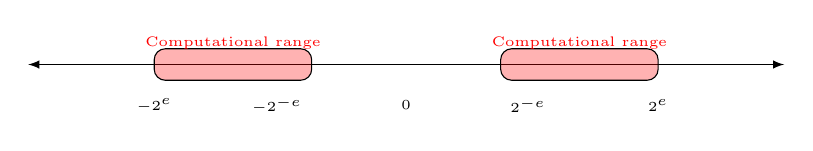
\begin{tikzpicture}[scale=0.4]
  \draw[latex-latex] (-12,0) -- (12,0);
  \draw[black, rounded corners, fill=red, fill opacity=0.3]
    (-8,-0.5) rectangle ++(5,1)
    node[anchor=south, midway, yshift=2pt, font=\tiny, align=center, color=red, opacity=1]
    {Computational range};
  \draw[black, rounded corners, fill=red, fill opacity=0.3]
    (3,-0.5) rectangle ++(5,1)
    node[anchor=south, midway, yshift=2pt, font=\tiny, align=center, color=red, opacity=1]
    {Computational range};
  \node[font=\tiny] at (-8,-1.3) {$-2^{e}$};
  \node[font=\tiny, anchor=east] at (-3,-1.3) {$-2^{-e}$};
  \node[font=\tiny] at (0,-1.3) {$0$};
  \node[font=\tiny, anchor=west] at (3,-1.3) {$2^{-e}$};
  \node[font=\tiny] at (8,-1.3) {$2^{e}$};
\end{tikzpicture}
\end{document}
